\subsection{IPFS}

Para realizar las métricas de IPFS, se utilizó el siguiente sistema:
\begin{itemize}
    \item \textbf{CPU:} Ryzen 5 1600
    \item \textbf{RAM:} 8GB
    \item \textbf{Almacenamiento:} SSD
\end{itemize}

\subsubsection{Costos}

Mientras que en una Blockchain convencional se delega el almacenamiento y cómputo en nodos dedicados a ese propósito a cambio de un monto monetaria, IPFS ejecuta todo de manera local. El costo de IPFS no es, entonces, monetario sino energético.

\subsubsection{Experiencia de desarrollo} % Developer Experience

\subsubsection{Aplicabilidad al caso de uso}

\subsubsection{Performance}

La performance en IPFS se ve afectada por algunas variables. Entre ellas se encuentran:

\begin{itemize}
    \item Uso de cache por parte de nodos de IPFS o gateways cuando se recupera un archivo.
    \item Cercanía al nodo correspondiente a la hora de publicar un CID en la Distributed Hash Table.
    \item Configuración y capacidades del nodo que tiene el contenido que se requiere.
    \item Cantidad de nodos alojando el contenido que se requiere.
\end{itemize}

 Se puede minimizar  el efecto de estas variables en la medida final sin distorsionar las métricas obtenidas. Más adelante se verán las maneras en las que se puede lidiar con estas variables.

\paragraph{Sitio Web Informativo}
La métrica que se decidió medir es la del \textbf{tiempo que tarda un nodo en desplegar un sitio web o contenido}. Para ello, se creó un clúster con un único nodo y un repositorio Git con contenido de distinta forma.

\subparagraph{Obtención de las métricas} En este caso, el proceso de despliegue se contiene dentro del contenedor \texttt{watcher}. Para medir el tiempo real que transcurre en cada paso del despliegue, se utilizó el comando de GNU \texttt{time} para cada paso, y el resultado es sumado para obtener el tiempo total que tardó desplegar el contenido.

\subparagraph{Variables consideradas} Las métricas obtenidas se lograron ajustando dos variables: el tamaño total del contenido, y la cantidad de archivos del mismo. Los archivos en sí fueron generados repitiendo un \texttt{UUID} hasta alcanzar el número de bytes deseados. Se utilizó este tipo de identificador para asegurar de que ningún archivo permanezca en alguna caché de la red o en la DHT, y a su vez no se repitan los CID entre archivos de la misma prueba.

\begin{figure}[H]
    \centering
    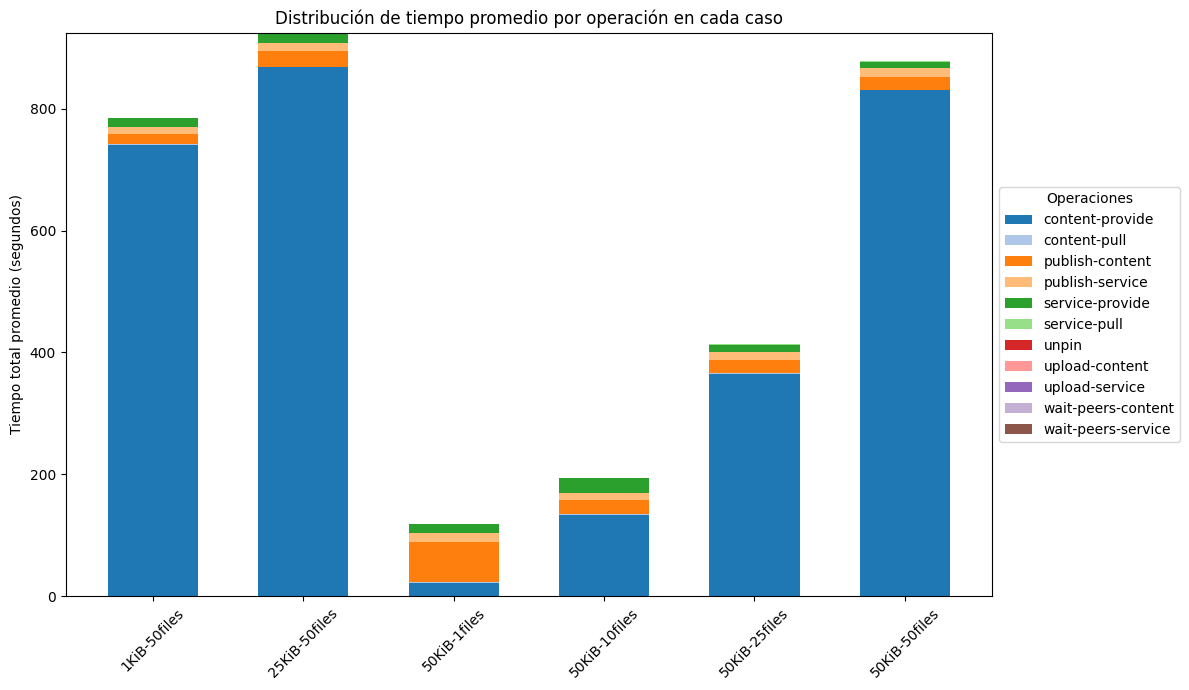
\includegraphics[width=1\linewidth]{img/metricas-ipfs/metricas-ipfs-caso1-1.png}
    \caption{Distribución del tiempo promedio para desplegar el contenido para cada caso}
    \label{fig:metricas-ipfs-caso1-1.png}
\end{figure}

De este gráfico podemos concluir que la operación más significante en términos de tiempo en el despliegue es la \textit{providing} del contenido. Esto es, la publicación de todos los CIDs en la DHT. Luego, le siguen el providing del \texttt{service.json}, y las operaciones para actualizar el valor al que apunta el nombre de IPNS, tanto del contenido como del \texttt{service.json}. Las demás operaciones se pueden despreciar.



\setlength\tabcolsep{10pt}
\begin{table}[!htbp]
    \centering
    \begin{tabular}{|c|c|c|c|c|c|}
    \hline
    & \textbf{Max} & \textbf{Mean} & \textbf{Min} & \textbf{Std} & \textbf{Median} \\
    \hline
    \textbf{1KiB-50files} & 23.65 s & 17.66 s & 7.70 s & 6.39 s & 21.71 s \\
    \hline
    \textbf{25KiB-50files} & 67.29 s & 25.92 s & 8.96 s & 15.24 s & 22.95 s \\
    \hline
    \textbf{50KiB-1files} & 78.75 s & 66.09 s & 61.48 s & 5.83 s & 62.93 s \\
    \hline
    \textbf{50KiB-10files} & 30.57 s & 12.93 s & 7.10 s & 7.42 s & 8.96 s \\
    \hline
    \textbf{50KiB-25files} & 23.79 s & 22.65 s & 21.94 s & 0.46 s & 22.57 s \\
    \hline
    \textbf{50KiB-50files} & 23.36 s & 20.95 s & 8.17 s & 4.27 s & 22.43 s \\
    \hline
    \end{tabular}
    \caption{Estadísticas para \texttt{publish-content}}
\end{table}

\setlength\tabcolsep{10pt}
\begin{table}[!htbp]
    \centering
    \begin{tabular}{|c|c|c|c|c|c|}
    \hline
    & \textbf{Max} & \textbf{Mean} & \textbf{Min} & \textbf{Std} & \textbf{Median} \\
    \hline
    \textbf{1KiB-50files} & 17.76 s & 10.30 s & 7.54 s & 3.39 s & 8.79 s \\
    \hline
    \textbf{25KiB-50files} & 23.03 s & 12.76 s & 7.31 s & 6.37 s & 8.74 s \\
    \hline
    \textbf{50KiB-1files} & 23.08 s & 15.37 s & 7.52 s & 6.71 s & 15.25 s \\
    \hline
    \textbf{50KiB-10files} & 23.31 s & 13.31 s & 7.34 s & 6.86 s & 8.44 s \\
    \hline
    \textbf{50KiB-25files} & 23.02 s & 12.17 s & 7.43 s & 5.80 s & 8.97 s \\
    \hline
    \textbf{50KiB-50files} & 22.85 s & 13.91 s & 7.28 s & 6.43 s & 11.32 s \\
    \hline
    \end{tabular}
    \caption{Estadísticas para \texttt{publish-service}}
\end{table}

\setlength\tabcolsep{10pt}
\begin{table}[!htbp]
    \centering
    \begin{tabular}{|c|c|c|c|c|c|}
    \hline
    & \textbf{Max} & \textbf{Mean} & \textbf{Min} & \textbf{Std} & \textbf{Median} \\
    \hline
    \textbf{1KiB-50files} & 851.26 s & 740.32 s & 682.64 s & 41.45 s & 734.15 s \\
    \hline
    \textbf{25KiB-50files} & 918.36 s & 868.11 s & 815.43 s & 26.57 s & 872.25 s \\
    \hline
    \textbf{50KiB-1files} & 42.09 s & 21.84 s & 10.79 s & 7.49 s & 20.14 s \\
    \hline
    \textbf{50KiB-10files} & 419.87 s & 372.47 s & 327.86 s & 25.09 s & 377.78 s \\
    \hline
    \textbf{50KiB-25files} & 412.30 s & 364.53 s & 306.15 s & 26.53 s & 366.01 s \\
    \hline
    \textbf{50KiB-50files} & 921.54 s & 830.06 s & 744.83 s & 41.12 s & 826.65 s \\
    \hline
    \end{tabular}
    \caption{Estadísticas para \texttt{content-provide}}
\end{table}

\setlength\tabcolsep{10pt}
\begin{table}[!htbp]
    \centering
    \begin{tabular}{|c|c|c|c|c|c|}
    \hline
    & \textbf{Max} & \textbf{Mean} & \textbf{Min} & \textbf{Std} & \textbf{Median} \\
    \hline
    \textbf{1KiB-50files} & 27.62 s & 14.83 s & 8.84 s & 6.12 s & 11.41 s \\
    \hline
    \textbf{25KiB-50files} & 34.34 s & 15.67 s & 10.99 s & 6.64 s & 11.66 s \\
    \hline
    \textbf{50KiB-1files} & 25.71 s & 13.63 s & 6.49 s & 5.26 s & 11.34 s \\
    \hline
    \textbf{50KiB-10files} & 20.88 s & 12.86 s & 10.84 s & 3.11 s & 11.30 s \\
    \hline
    \textbf{50KiB-25files} & 20.78 s & 12.42 s & 9.78 s & 3.47 s & 11.26 s \\
    \hline
    \textbf{50KiB-50files} & 20.27 s & 11.31 s & 6.82 s & 3.17 s & 10.97 s \\
    \hline
    \end{tabular}
    \caption{Estadísticas para \texttt{service-provide}}
\end{table}

Teniendo en cuenta esto, se puede observar cuál es la causa de la variación del tiempo de providing ajustando las dos variables mencionadas.

\begin{figure}[H]
    \centering
    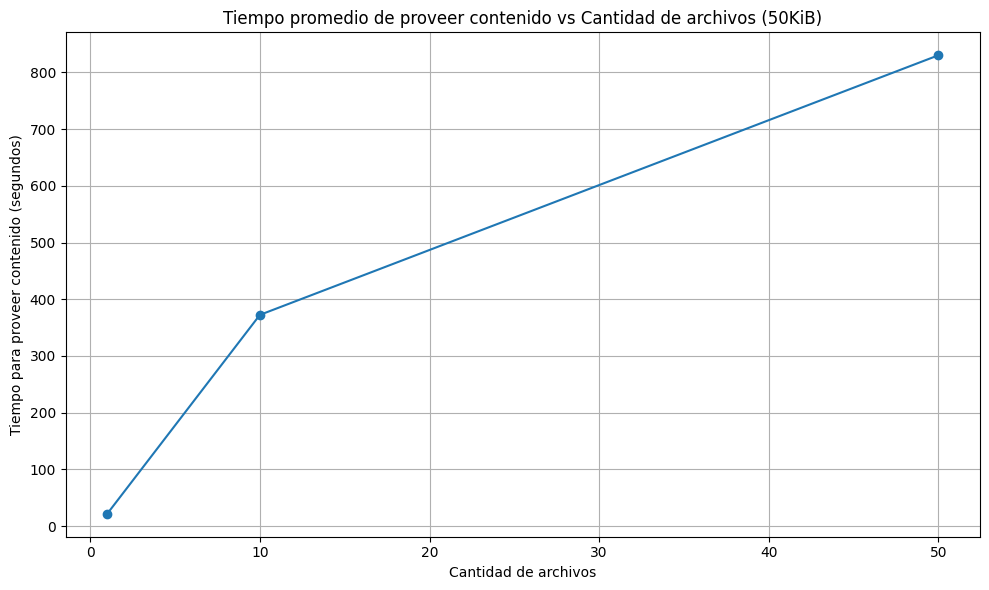
\includegraphics[width=1\linewidth]{img/metricas-ipfs/tiempo-por-cant-archivos.png}
    \caption{Tiempo promedio por cantidad de archivos}
    \label{fig:tiempo-por-cant-archivos.png}
\end{figure}

\begin{figure}[H]
    \centering
    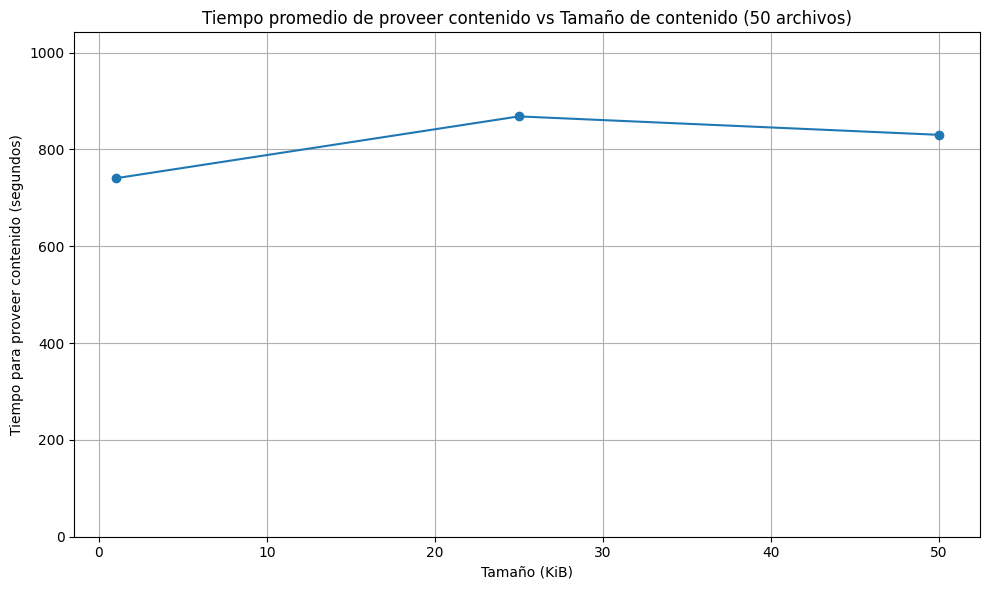
\includegraphics[width=1\linewidth]{img/metricas-ipfs/tiempo-por-tamano.png}
    \caption{Tiempo promedio por tamaño del contenido}
    \label{fig:tiempo-por-tamano.png}
\end{figure}

La cantidad de archivos que tiene el contenido a publicar es la variable que modifica drásticamente el tiempo que tarda un nodo confiable para desplegarlo, como se ve en las figuras. Esto se debe a que la publicación del CID del directorio no es suficiente para que otro nodo pueda obtener el contenido de ese directorio. En cambio, se requiere que se publique todos los archivos y directorios que componen el contenido. Esto también se demuestra con el tiempo constante para publicar el archivo \texttt{service.json}, ya que en todos los casos sigue siendo un sólo archivo. 

\begin{figure}[H]
    \centering
    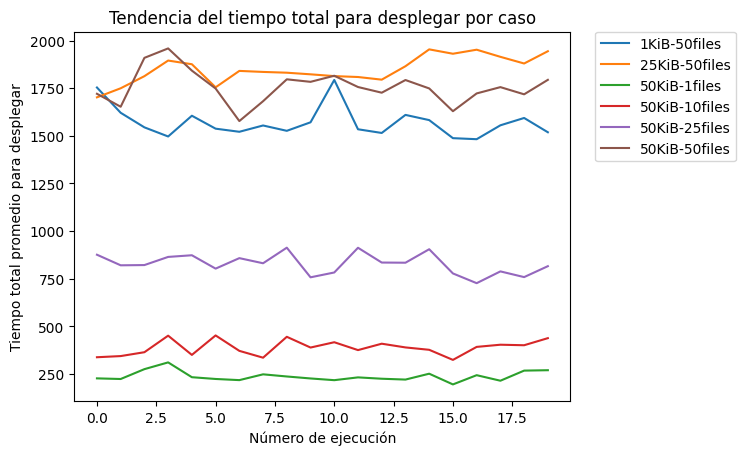
\includegraphics[width=0.9\linewidth]{img/metricas-ipfs/tendencia-desplegar.png}
    \caption{Tendencia del tiempo total promedio para desplegar el contenido en ejecuciones consecutivas.}
    \label{fig:tendencia-desplegar.png}
\end{figure}

Por último, se ve como la tendencia en ejecuciones consecutivas no afecta el tiempo que se tarda en desplegar.

\paragraph{Repositorio de conocimiento}

Las métricas tanto de Astrawiki como Astrachat se ven muy relacionadas, debido a que el grueso del trabajo relacionado a IPFS se realiza con su biblioteca en común, AstraDB. Por ejemplo, el tiempo que tarda un nodo en obtener una nueva versión de un articulo es el similar al que tarda un nodo en recibir un mensaje. Por ello, se prefirió complementar las métricas obtenidas para acentuar el uso específico de AstraDB de cada caso de uso, y evitar métricas repetidas. 

\paragraph{Mensajero en tiempo real}

Las siguientes métricas se obtuvieron con un nodo colaborador y un nodo común. Se levantaron ambos nodos en la misma máquina para poder coordinar ambos nodos y facilitar la obtención de métricas.

Se asume una conexión existente entre el nodo colaborador y el nodo común. Para agilizar la obtención de métricas la conexión directamente mediante las multiaddresses de los nodos, aunque en un caso real se debería encontrar utilizando la DHT. Una vez establecida la conexión el uso es el mismo, por lo que estas métricas no dependen del tipo de mecanismo utilizado para el establecimiento de la conexión.

\subparagraph{Tiempo en enviar un mensaje}

A continuación se muestran los resultados de medir el tiempo que le lleva a un nodo enviar un mensaje a un chat. Para este caso, se asume que el nodo ya está conectado, situación a la que debería llegar un usuario de todos modos antes de enviar un mensaje.

\setlength\tabcolsep{10pt}
\begin{table}[!htbp]
    \centering
    \begin{tabular}{|l|c|c|c|c|c|}
        \hline
        & \textbf{Max} & \textbf{Mean} & \textbf{Min} & \textbf{Std} & \textbf{Median} \\ \hline
        \textbf{short} & 24230 ms & 185.1 ms & 30.25 ms & 765.3 ms & 161.4 ms \\ \hline
        \textbf{medium} & 21870 ms & 175.8 ms & 26.44 ms & 690.1 ms & 153.4 ms \\ \hline
        \textbf{large} & 121000 ms & 265.5 ms & 20.59 ms & 3822 ms & 145.5 ms \\ \hline
    \end{tabular}
    \caption{Tiempo en enviar un mensaje}
\end{table}

Algo a notar son los máximos para cada medición. Estos se deben a una pérdida en la conexión entre nodos que puede ocurrir en el transcurso de una sesión. Sin embargo, son pocos los casos dado el tamaño de la muestra. Por otro lado, el tamaño del mensaje no afecta de forma apreciable el tiempo de envío.

\subparagraph{Tiempo en obtener mensajes}

El gráfico presenta cómo varía el tiempo de respuesta, medido en milisegundos, a medida que crece la cantidad de mensajes en un chat, desde 0 hasta 1000 mensajes en el chat. Se consideran tres tipos de mensajes, y se observa un incremento progresivo en el tiempo necesario para obtenerlos. Esta métrica se obtuvo midiendo el tiempo requerido para recuperar todos los mensajes en chats con diferentes tamaño de contenido. Además, se eliminaron los \textit{outliers} por pérdida de conexión para poder visualizar mejor la tendencia en general.

\begin{figure}[h!]
    \centering
    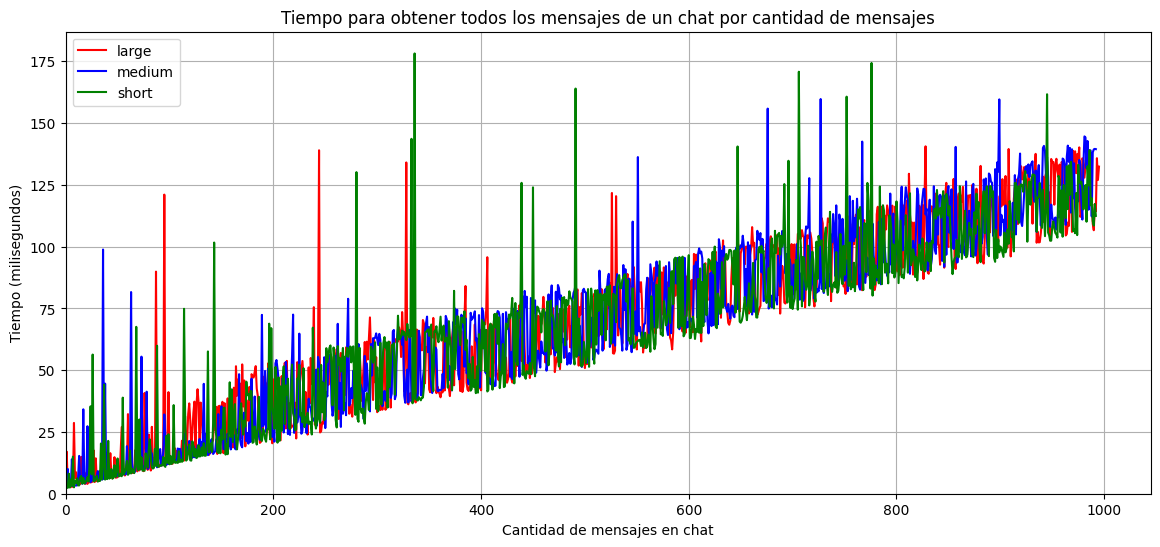
\includegraphics[width=1\linewidth]{img/metricas-ipfs/tiempo-para-obtener-por-cant-msjs.png}
    \caption{Tiempo para obtener mensajes de un chat según el tamaño del chat}
    \label{fig:ipfs-get-message-graphic.png}
\end{figure}

\setlength\tabcolsep{10pt}
\begin{table}[!htbp]
    \centering
    \begin{tabular}{|l|c|c|c|c|c|}
        \hline
        & \textbf{Max} & \textbf{Mean} & \textbf{Min} & \textbf{Std} & \textbf{Median} \\ \hline
        \textbf{short} & 5665 ms & 79.45 ms & 2.340 ms & 248.8 ms & 69.19 ms \\ \hline
        \textbf{medium} & 8471 ms & 85.47 ms & 2.718 ms & 359.4 ms & 70.14 ms \\ \hline
        \textbf{large} & 3905 ms & 76.96 ms & 2.642 ms & 161.2 ms & 69.15 ms \\ \hline
    \end{tabular}
    \caption{Tiempo en obtener mensajes}
\end{table}  

\subparagraph{Tiempo entre enviar y recibir un mensaje}

Esta métrica calcula el tiempo que tarda el nodo común en recibir un mensaje enviado por el nodo colaborador. Para ello se utiliza el \texttt{EventEmitter} integrado en Astrachat, logrando una medición exacta del trayecto de un mensaje para una conexión ya establecida. Al igual que en los demás casos, existen outliers provenientes de pérdidas de conexión, los cuáles se pueden observar en los máximos obtenidos. Sin embargo, la desviación estándar y el valor promedio y mediano indican que estos no son frecuentes.

\setlength\tabcolsep{10pt}
\begin{table}[!htbp]
    \centering
    \begin{tabular}{|l|c|c|c|c|c|}
        \hline
        & \textbf{Max} & \textbf{Mean} & \textbf{Min} & \textbf{Std} & \textbf{Median} \\ \hline
        \textbf{short} & 22790 ms & 298.1 ms & 47.85 ms & 1341 ms & 198.8 ms \\ \hline
        \textbf{medium} & 18050 ms & 227.0 ms & 40.89 ms & 800.4 ms & 195.0 ms \\ \hline
        \textbf{large} & 20680 ms & 285.8 ms & 64.47 ms & 1264 ms & 196.1 ms \\ \hline
    \end{tabular}
    \caption{Tiempo entre enviar y recibir un mensaje}
\end{table}  